% Drawing 64/01-5 -- folder 64, batch 01, archive page 13 (PDF page 14).
% Transcription: marge gauche, en bas : un carré de sommets $s'$ (en haut à gauche) et $s$ (en haut à droite, gros point), l'arête supérieure $a$ épaissie, l'arête droite marquée $a'$ ; au-dessus, une flèche droite allant de droite à gauche et une flèche courbe descendant à droite de $s$ ; un mot biffé au-dessus des flèches.
% Kind: square with a heavy edge and two arrows (the two opposite rotations). Method 2 (schematic redraw from the facsimile). Status: ok.
% Notes: As on the page: the square, its upper edge a heavy, from s' (upper left) to s (upper right, heavy point), the right edge marked a'; above it a straight arrow pointing left, and from the same place a curved arrow that goes down at the right of s. Left out: the struck word above the arrows (not drawn, as struck material). Disagreement in part with the note of the transcription, which speaks of one curved arrow above s: the page has two arrows, one straight to the left (s to s') and one curved downwards (a to a'). Redrawn 2026-11-12 (issue 128): to check again.
% Coordinates: 1 unit = 0.5 mm = 1/100 of the crop width (bbox in page fractions: [0.15, 0.7, 0.31, 0.83]).
% Redrawn by Claude (claude-fable-5-2), issue #128, 2026-11-12; not checked by a human; not compiled (no TeX in the session).
% Rights: reproduces part of the work -- behind RENDER_TRANSCRIPTS, never published by itself.
\documentclass[tikz,border=3pt]{standalone}
\usepackage{amsmath,amssymb}
\usetikzlibrary{patterns,arrows.meta}
\tikzset{pencil/.style={black!45}, struck/.style={black!35}, mpt/.style={circle,draw,inner sep=1.3pt}, pt/.style={circle,fill,inner sep=0.9pt}, opt/.style={circle,draw,fill=white,inner sep=1.1pt}}
\begin{document}
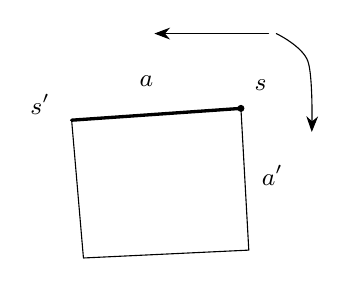
\begin{tikzpicture}[x=0.5mm,y=0.5mm,line cap=round,line join=round,font=\scriptsize]
\draw[very thick] (21,-45) -- (64,-42);
\draw (64,-42) -- (66,-78) -- (24,-80) -- (21,-45);
\node[pt] at (64,-42) {};
\draw[-{Stealth[length=2mm]}] (71,-23) -- (42,-23);
\draw[-{Stealth[length=2mm]}] plot[smooth, tension=0.55] coordinates {(73,-23) (81,-30) (82,-48)};
\node[inner sep=1pt] at (13,-41) {\small $s'$};
\node[inner sep=1pt] at (40,-35) {\small $a$};
\node[inner sep=1pt] at (69,-36) {\small $s$};
\node[inner sep=1pt] at (72,-59) {\small $a'$};
\end{tikzpicture}
\end{document}
